%% RADiCAL Paper 1 (timing) -- NIM A (Elsevier elsarticle) two-column style.
%% Compile: tectonic radical_timing.tex
%% NOTE: the author block is a PLACEHOLDER; complete it with the full RADiCAL author
%% list (as in Ref.~[2], NIM A 1068 (2024) 169737, p.1) before submission.
\documentclass[final,5p,times,twocolumn]{elsarticle}

\usepackage{graphicx}
\usepackage{amsmath}
\usepackage{booktabs}
\usepackage{xcolor}
\graphicspath{{figs/}}

\journal{Nuclear Instruments and Methods in Physics Research A}

\begin{document}

\begin{frontmatter}

\title{Light yield, not wavelength-shifter species, sets the time resolution
of RADiCAL sampling-calorimeter modules}

%% ---- Author block. Lead author J. Wetzel for Paper 1 (collaboration sets the full
%% author ORDER). The 39-author RADiCAL roster + 11 affiliations are verified in Ref.~[2]
%% (NIM A 1068 (2024) 169737). Affiliations there: a Adiyaman U.; b Caltech; c Coe College;
%% d Hofstra U.; e U. Iowa; f Istanbul U.; g Istanbul U.-Cerrahpasa; h Istanbul Technical U.;
%% i U. Notre Dame; j U. Virginia; k Yildiz Technical U.
\author[uiowa]{J.~Wetzel\corref{cor}}
\ead{james@animal-lamps.com}
\cortext[cor]{Corresponding author.}
\author[radical]{\textit{for the RADiCAL Collaboration}}
\affiliation[uiowa]{organization={University of Iowa},
            city={Iowa City}, state={IA}, country={USA}}
\affiliation[radical]{organization={RADiCAL Collaboration}}
%% ---------------------------------------------------------------------------

\begin{abstract}
We compare the precision-timing performance of four builds of the RADiCAL
tungsten/LYSO:Ce sampling electromagnetic calorimeter module that differ primarily
in their wavelength-shifter (WLS) capillaries -- the common LYSO:Ce scintillator and
tungsten absorber are unchanged -- exposed to $25$--$150$~GeV electrons at the CERN
SPS: a high-light DSB1 (organic WLS) build, a low-light LuAG:Ce (ceramic WLS) build,
a mixed DSB1/LuAG:Ce build, and a multi-segment build. The high-gain channels used for timing saturate,
clipping at $820$~mV; we recover the unclipped rising edge event by event from a
linear low-gain copy of each pulse, timing a constant fraction of the
low-gain-predicted true peak on an edge a factor $\sim3.7$ steeper than the
clipped-peak foot, which improves the resolution by a few picoseconds over timing the
clipped pulse. Using a microchannel-plate-free differential estimator,
$(\mathrm{DW}-\mathrm{UP})/2$, formed from the four upstream and four downstream
silicon-photomultiplier readouts, we measure the time resolution of every build and
parametrise it as $\sigma_t = a/\sqrt{E}\oplus b$. The stochastic term $a$ scales
with the collected scintillation light, more than doubling from the high-light to the
low-light build, whereas the floor $b\approx20$~ps is consistent across the
LYSO-based builds and with the value previously reported for DSB1
[NIM A \textbf{1068} (2024) 169737]. The time resolution is therefore governed by
light yield, not by the wavelength-shifter species: at equal light all materials
approach the same floor. The high-light build reaches $25.4$~ps for the brightest
$150$~GeV showers. We discuss light yield as the primary design lever and the
material-independent floor as shared shower/detector physics.
\end{abstract}

\begin{keyword}
Fast timing \sep Sampling calorimeter \sep LYSO \sep LuAG:Ce \sep Wavelength shifter \sep
Silicon photomultiplier \sep Signal saturation \sep 4D calorimetry
\end{keyword}

\end{frontmatter}

%======================================================================
\section{Introduction}
\label{sec:intro}

Future high-luminosity colliders demand electromagnetic (EM) calorimeters that resolve
the \emph{time} of a shower to a few tens of picoseconds, in addition to its energy,
to associate deposits with the correct primary vertex and reject out-of-time
pile-up~\cite{cmsmtd}. The RADiCAL R\&D programme develops ultra-compact,
radiation-hard sampling EM calorimeter modules toward this goal~\cite{radical}.

A first RADiCAL test-beam measurement, on a single high-light build, reported a time
resolution of $\approx\!27$~ps at $150$~GeV and parametrised the energy dependence as
$\sigma_t = a/\sqrt{E}\oplus b$ with $a=256$~ps$\sqrt{\mathrm{GeV}}$ and a floor
$b=17.5$~ps~\cite{radical}. That work also identified, as a priority for further study
(its Section~7), a direct comparison of the timing performance of different
wavelength-shifter (WLS) scintillator materials in otherwise-identical modules. This
paper presents that comparison.

The central question is whether a lower-light WLS material such as LuAG:Ce times worse
than the high-light organic DSB1 because of the \emph{species} of scintillator --- its
emission spectrum, decay time, or refractive index --- or simply because it collects
\emph{less light}. The distinction matters for detector design: if light yield is the
sole driver, the timing of any candidate material is predictable from its light output,
and the material can be chosen for radiation hardness or mechanical properties without a
separate timing penalty. We answer it by measuring four builds spanning a factor
$\sim2$ in light yield with a common analysis, and by separating the light-dependent
stochastic term from the irreducible floor.

A prerequisite is to time all builds on an equal footing despite saturation of the
front end. We therefore first describe a high-gain/low-gain (HG/LG) ratio method that
recovers the saturated rising edge (Section~\ref{sec:method}), then the estimator and
selection (Section~\ref{sec:estimator}), and finally the results
(Section~\ref{sec:results}): the four-build time resolution, its decomposition into a
light-driven stochastic term and a material-independent floor, and the implications.

%======================================================================
\section{Experimental setup}
\label{sec:setup}

\subsection{Module and builds}
The module is a tungsten/LYSO:Ce sampling calorimeter of the ``shashlik'' type:
alternating plates of tungsten absorber and cerium-doped lutetium--yttrium
oxyorthosilicate (LYSO:Ce) scintillator, $\approx\!25$ radiation lengths deep, read out
longitudinally by WLS capillaries. Four capillaries traverse the stack and are each read
out at both ends, giving $4\times2 = 8$ silicon-photomultiplier (SiPM) channels; we
label the four downstream ends collectively DW and the four upstream ends UP. The
transverse position of each incident electron is measured by a wire chamber and used to
define a fiducial region on the beam spot.

Four builds were exposed, differing primarily in the WLS material of the capillaries --
and hence in light yield -- while sharing the same LYSO:Ce scintillator and tungsten
absorber (Table~\ref{tab:builds}): \textbf{DSB1}, high-light organic WLS;
\textbf{LUAG}, low-light ceramic LuAG:Ce WLS; \textbf{MIXED}, a single module combining
DSB1 and LuAG:Ce capillaries on opposite diagonals; and \textbf{TENERGY}, a
multi-segment high-light build with an added longitudinal energy-readout section. DSB1,
the brightest, is the build of Ref.~\cite{radical}.

\subsection{Readout, beam, and reference}
Each SiPM signal is split into a high-gain (HG) copy, optimised for timing, and a
low-gain (LG) copy, optimised for energy linearity, both digitised by DRS4
switched-capacitor waveform digitisers (CAEN DT5742)~\cite{drs4} at $5$~GS/s over a
1024-cell window, with per-cell calibration applied offline. The HG channels clip at
$\approx\!820$~mV; the LG channels remain linear. Measurements used a $25$--$150$~GeV
electron beam at the CERN SPS (May 2023); DSB1 was run at all six energies in $25$~GeV
steps, the other builds at $50$--$150$~GeV. A microchannel-plate photomultiplier
(MCP-PMT) provides a common start; all per-channel times are MCP-referenced, and the
differential estimator below cancels this reference.

%======================================================================
\section{Recovering the saturated edge: the HG/LG-ratio method}
\label{sec:method}

Precision timing of all builds on an equal footing requires the same well-defined edge
in each, but the HG timing pulses saturate. The recorded HG amplitude piles up at the
$820$~mV clip (Fig.~\ref{fig:clip}); for all but the smallest showers the waveform is
flat across its maximum, and a constant-fraction discriminator (CFD) referenced to the
measured peak is forced onto the shallow foot of the pulse, where the slope --- and the
timing information --- is poor.

\begin{figure}[t]
\centering
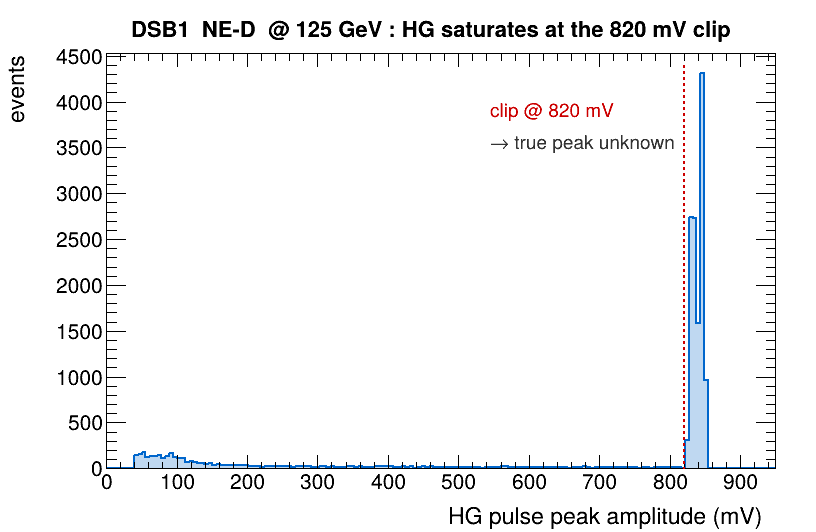
\includegraphics[width=0.92\linewidth]{clip.png}
\caption{Distribution of recorded high-gain pulse-peak amplitudes (one channel,
$125$~GeV). The pile-up at $\approx\!820$~mV is the digitiser clip: most showers
saturate, so the true peak --- and the steep edge that leads to it --- is not directly
recorded.}
\label{fig:clip}
\end{figure}

The LG copy, though too small for precise timing alone, is linear and therefore measures
the true amplitude the HG channel would have reached. We use a per-end calibration
\begin{equation}
  \mathrm{HG}_\mathrm{true} = a_\mathrm{c} + b_\mathrm{c}\,\mathrm{LG}_\mathrm{peak},
  \label{eq:hglg}
\end{equation}
fit on the unsaturated population (Fig.~\ref{fig:hglg}), to predict the unclipped HG
peak event by event. A CFD threshold is then placed at a fixed fraction ($15\%$) of this
\emph{predicted} peak and applied to the recorded HG waveform; because the predicted
peak lies far above the clip, the threshold sits on the steep, unsaturated edge. We call
the resulting MCP-referenced crossing time \texttt{hg\_lgcfd}.

\begin{figure*}[t]
\centering

\includegraphics[width=0.96\linewidth]{hglg.png}
\caption{High-gain versus low-gain pulse-peak amplitude for the eight readout channels
($100$~GeV). The high-gain response saturates at $820$~mV (horizontal band) while the
low-gain copy remains linear; the per-channel linear fit (red line), Eq.~(\ref{eq:hglg}),
predicts the unclipped true peak.}
\label{fig:hglg}
\end{figure*}

\begin{figure}[t]
\centering

\includegraphics[width=\linewidth]{pulse.png}
\caption{A single saturated high-gain waveform ($125$~GeV). The recorded pulse clips at
$820$~mV (grey); the low-gain copy predicts a true peak of $1997$~mV (green). The CFD at
$15\%$ of the predicted peak (\texttt{hg\_lgcfd}, blue) times an edge of $381$~mV/ns,
against $102$~mV/ns at the clipped-peak foot where the $5\%$ CFD (\texttt{cfd05}, red)
must sit --- a factor $3.7$ steeper.}
\label{fig:pulse}
\end{figure}

The recovered edge is a factor $\sim\!3.7$ steeper than the clipped-peak foot
(Fig.~\ref{fig:pulse}: $381$ vs $102$~mV/ns). Since the slew contribution to the time
resolution scales as $\sigma_t \simeq \sigma_V/(\mathrm{d}V/\mathrm{d}t)$ with
$\sigma_V$ the voltage noise, a steeper edge directly improves timing. The method is
applied uniformly to every build. For the low-light builds (LuAG, TENERGY), whose small
pulses can defeat the fractional-threshold reconstruction, a robust fixed-threshold
leading-edge time is used instead; the choice of per-build timing source is noted in
Table~\ref{tab:builds}.

%======================================================================
\section{Timing estimator and event selection}
\label{sec:estimator}

For each event we form the per-end mean crossing time and combine the two ends into the
differential estimator
\begin{equation}
  t_{\mathrm{DW-UP}} \equiv \tfrac{1}{2}\!\left(\bar t_\mathrm{DW} - \bar t_\mathrm{UP}\right),
  \label{eq:dwup}
\end{equation}
averaging up to four downstream and four upstream SiPM times. The difference cancels any
time common to both ends --- in particular the MCP start --- so $t_{\mathrm{DW-UP}}$ is
free of the reference jitter; averaging four channels per end suppresses uncorrelated
single-channel noise. The single-event resolution quoted throughout is the standard
deviation of a Gaussian fit to the \emph{central peak} of the $t_{\mathrm{DW-UP}}$
distribution; a small non-Gaussian shoulder (the $\sim\!0.2$~ns satellite also noted in
Ref.~\cite{radical}) is excluded from the fit and has negligible effect on the quoted
width.

Events are required to lie in the wire-chamber fiducial region and to have a valid MCP
signal. Because shower fluctuations spread the collected light at fixed beam energy, the
resolution depends on shower brightness; for a uniform, well-measured comparison across
builds we quote the resolution of the $1000$ brightest showers (by total low-gain signal)
at each energy, which fixes the statistical precision of every point. Within each build,
the resolution improves with shower brightness, as expected from the slew argument.

%======================================================================
\section{Results}
\label{sec:results}

\subsection{Timing distributions}
Figure~\ref{fig:dist} shows, for DSB1 with all energies pooled and binned by amplitude,
the $t_{\mathrm{DW-UP}}$ (top) and absolute $(\mathrm{DW}+\mathrm{UP})/2$ (middle)
distributions with their central-peak Gaussian fits, and the fitted $\sigma_t$ versus
amplitude (bottom). The distributions are clean and single-peaked at every amplitude;
the differential estimator is consistently narrower than the absolute one, as expected
once the common-mode reference jitter is removed, and the width falls monotonically with
shower brightness.

\begin{figure*}[t]
\centering

\includegraphics[width=0.98\linewidth]{dist.png}
\caption{DSB1 timing distributions, all energies pooled and binned by amplitude. Top:
$(\mathrm{DW}-\mathrm{UP})/2$ (MCP-free). Middle: $(\mathrm{DW}+\mathrm{UP})/2$
(absolute). Each $\sigma$ (ps) is the central-peak Gaussian fit. Bottom: the fitted
$\sigma_t$ versus amplitude. The peaks are clean Gaussians at every brightness.}
\label{fig:dist}
\end{figure*}

\subsection{Light yield sets the resolution}
\label{sec:thesis}
Figure~\ref{fig:thesis} is the central result. For each build, the brightest-shower
$\sigma_t$ is plotted against beam energy and fit to the published form
\begin{equation}
  \sigma_t(E) = \frac{a}{\sqrt{E}} \oplus b,
  \label{eq:fit}
\end{equation}
with $a$ the (light-driven) stochastic term and $b$ the floor as $E\to\infty$. The
fitted parameters are collected in Table~\ref{tab:builds}. Two features stand out.
First, the builds order cleanly by light yield, and the \emph{stochastic} term tracks it:
$a$ rises from $201$~ps$\sqrt{\mathrm{GeV}}$ for high-light DSB1 to
$455$~ps$\sqrt{\mathrm{GeV}}$ for low-light LuAG, a factor of $2.3$. Second, the
\emph{floor} $b$ is consistent across the LYSO-based builds --- $20\pm1$ (DSB1),
$22\pm3$ (TENERGY), $20\pm6$~ps (LuAG) --- and agrees with the $17.5$~ps reported for
DSB1 in Ref.~\cite{radical}. (MIXED sits higher, $b=35\pm2$~ps; its low-gain readout is
partly compromised, so its energy axis carries a systematic and its floor is
indicative.) The energy dependence is well described by the $1/\sqrt{E}$ (photostatistics)
form ($\chi^2/\mathrm{ndf}\approx2$); a $1/E$ (pure-slew) form fits markedly worse.

\begin{figure}[t]
\centering
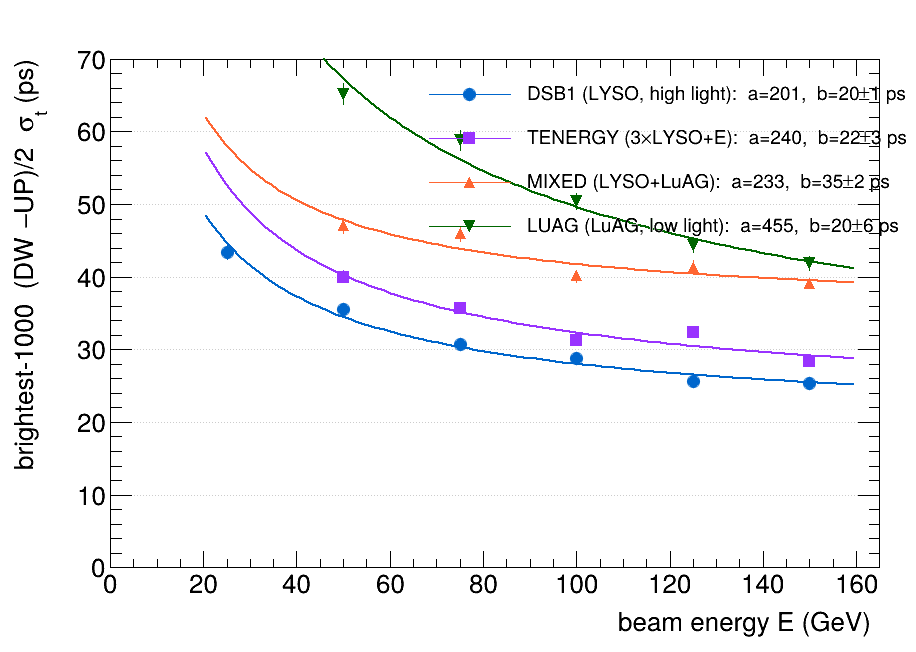
\includegraphics[width=\linewidth]{thesis.png}
\caption{Brightest-shower $(\mathrm{DW}-\mathrm{UP})/2$ time resolution versus beam
energy for the four builds, each fit to $\sigma_t=a/\sqrt{E}\oplus b$
[Eq.~(\ref{eq:fit})]. The stochastic term $a$ tracks light yield (DSB1 lowest, LuAG
highest); the floor $b\approx20$~ps is consistent across the LYSO builds (MIXED, with a
compromised low-gain readout, excepted).}
\label{fig:thesis}
\end{figure}

\begin{table}[t]
\centering
\caption{Per-build fit of $\sigma_t=a/\sqrt{E}\oplus b$ to the brightest-shower
resolution, the timing source used, and the best resolution measured at $150$~GeV. The
WLS column gives the wavelength-shifter material of the capillaries; the LYSO:Ce
scintillator and tungsten absorber are common to every build. The published DSB1 values
(cfd05) are shown for comparison.}
\label{tab:builds}
\small
\begin{tabular}{lccccc}
\toprule
Build & WLS & src & $a$ & $b$ (ps) & $\sigma_t^{150}$ \\
\midrule
DSB1     & organic, hi   & lgcfd & $201$ & $20\pm1$ & $25.4$ \\
TENERGY  & organic, seg  & led   & $240$ & $22\pm3$ & $28.7$ \\
MIXED    & org.+cer.     & lgcfd & $233$ & $35\pm2$ & $40.0$ \\
LUAG     & ceramic, lo   & led   & $455$ & $20\pm6$ & $41.2$ \\
\midrule
DSB1\,\cite{radical} & organic & cfd05 & $256$ & $17.5$ & $27$ \\
\bottomrule
\end{tabular}
\end{table}

The interpretation is direct: \textbf{light yield sets the dominant, material-dependent
(stochastic) part of the time resolution, while the floor is a shared, material-independent
limit.} A lower-light material times worse only in proportion to its reduced light; at
sufficient light any of these materials approaches the same $\sim\!20$~ps floor. The
choice of WLS species per se is not a timing penalty.

\subsection{The gain from recovering the edge}
\label{sec:method-gain}
The benefit of the HG/LG-ratio method is isolated by a direct comparison on
\emph{identical} showers (Fig.~\ref{fig:method}): the brightest-$1000$ DSB1 resolution
is computed with cfd05 (a CFD on the clipped measured peak, as in Ref.~\cite{radical})
and with \texttt{hg\_lgcfd} (the recovered edge), the selection and estimator held fixed
so that only the per-channel time differs. Timing the recovered edge improves the
resolution by $3.1$~ps at $150$~GeV and lowers the floor from $22.1\pm1.8$ to
$19.5\pm1.1$~ps. The gain is energy-dependent, largest where the timing is hardest: at
high energy, where saturation is most severe, and at the lowest energy, where the $5\%$
foot of a small pulse sits in noise; it is negligible at $50$--$75$~GeV. The stochastic
term is essentially unchanged ($a=205\to201$~ps$\sqrt{\mathrm{GeV}}$), so the method acts
chiefly on the high-energy/floor regime. (The cfd05 value here, $a=205$, reflects the
brightest-shower selection of this controlled comparison and differs from the $256$ of
Ref.~\cite{radical} in Table~\ref{tab:builds}, which used a different selection; holding
the selection fixed isolates the timing method.) The best single-event resolution
measured, for the brightest $150$~GeV DSB1 showers, is $25.4$~ps.

\begin{figure}[t]
\centering
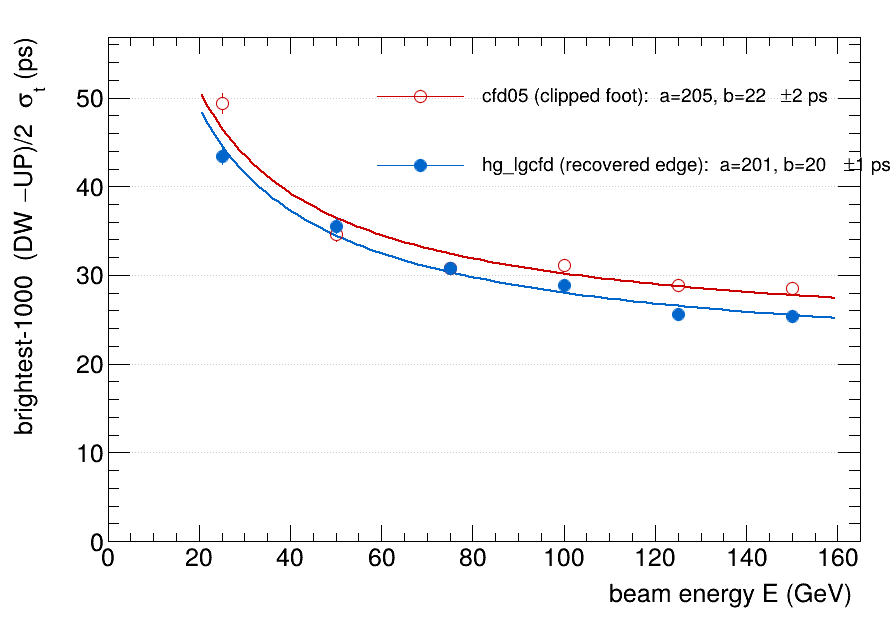
\includegraphics[width=\linewidth]{method.png}
\caption{Time resolution of the brightest-$1000$ DSB1 showers timed with cfd05 (CFD on
the clipped foot, open) and \texttt{hg\_lgcfd} (CFD on the LG-recovered edge, filled),
identical events and selection. Recovering the edge improves the resolution by $\sim3$~ps
at $150$~GeV and lowers the floor.}
\label{fig:method}
\end{figure}

\subsection{Systematic uncertainties}
\label{sec:syst}
The headline brightest-$1000$ $(\mathrm{DW}-\mathrm{UP})/2$ resolution was recomputed
under deliberate variations of every selection knob, on the adopted timing source:
the brightness selection ($K=500$ and $2000$ versus the nominal $1000$), the timing
fiducial radius ($2.5$ and $3.5$ versus $3.0$~mm), the MCP saturation window (upper cut
$700$ versus $750$~mV), the per-channel HG threshold ($30$ versus $20$~mV), and the
fit energy range ($50$--$150$ versus $25$--$150$~GeV). The shifts are collected in
Table~\ref{tab:syst}, with the total systematic taken as their RMS. The selection
values themselves were fixed by the scans of Appendix~\ref{app:opt}
(Fig.~\ref{fig:opt}); the timing-method choice (cfd05 versus the recovered edge) is the
subject of Sec.~\ref{sec:method-gain} and is not folded into this budget.

The headline is robust: the total selection systematic on $\sigma_t(150)$ is
$\le\!1$~ps for the high-light builds (DSB1, TENERGY) and $\sim\!1.5$~ps for MIXED and
LUAG. The dominant single variation is loosening the brightness selection to $K=2000$,
which admits dimmer showers and genuinely degrades the resolution by $2$--$2.4$~ps --- a
manifestation of the same light--resolution dependence that is the paper's subject,
not an analysis artefact. Crucially, the floor is stable: for DSB1,
$b=19.5\pm1.1\,(\mathrm{stat})\pm1.2\,(\mathrm{syst})$~ps, and across the LYSO builds
$b$ stays near $20$~ps (TENERGY $21.6$, LUAG $19.8$) within the combined uncertainty, so
the agreement with the published $17.5$~ps survives the systematic variations. The
elevated floor of the MIXED build ($34.6$~ps) is a distinct feature of that compromised
configuration and carries the largest systematic, but does not affect the shared-floor
conclusion drawn from the uniform builds.

%======================================================================
% auto-generated by analyze/studies/paperSystematics.C
\begin{table}[t]
\centering
\caption{Systematic budget for the brightest-1000 $(\mathrm{DW}-\mathrm{UP})/2$ time
resolution. Each row recomputes $\sigma_t(150)$ and the fit floor $b$ under one
selection variation; the entry is the shift from the nominal value (ps). The total
systematic is the RMS of the shifts; the statistical floor error is from the fit. The
timing-method choice (cfd05 vs.\ the recovered edge) is the subject of
Sec.~\ref{sec:method-gain} and is not folded in here.}
\label{tab:syst}
\small
\begin{tabular}{lcccc}
\toprule
Variation & DSB1 & TENERGY & MIXED & LUAG \\
\midrule
\multicolumn{5}{l}{\emph{shift in }$\sigma_t(150)$\emph{ [ps]}}\\
$K{=}500$ & $+0.1$ & $-0.3$ & $-1.0$ & $+0.8$ \\
$K{=}2000$ & $+2.1$ & $+2.4$ & $+2.3$ & $+0.4$ \\
$r_{\mathrm{fid}}{=}2.5$~mm & $+1.2$ & $+0.3$ & $-0.7$ & $-1.1$ \\
$r_{\mathrm{fid}}{=}3.5$~mm & $+0.2$ & $+0.6$ & $+2.0$ & $+3.8$ \\
MCP${}<700$~mV & $+0.3$ & $+0.2$ & $+2.5$ & $-0.7$ \\
HG${}>30$~mV & $+0.0$ & $-0.0$ & $+0.0$ & $+0.0$ \\
fit $50$--$150$ only & $+0.0$ & $+0.0$ & $+0.0$ & $+0.0$ \\
\midrule
nominal $\sigma_t(150)$ & $25.3$ & $28.3$ & $39.1$ & $41.9$ \\
total syst. & $\pm0.9$ & $\pm0.9$ & $\pm1.5$ & $\pm1.6$ \\
\midrule
floor $b$ (nom) & $19.5$ & $21.6$ & $34.6$ & $19.8$ \\
$b$ syst. & $\pm1.2$ & $\pm2.2$ & $\pm2.2$ & $\pm2.4$ \\
$b$ stat. & $\pm1.1$ & $\pm2.7$ & $\pm2.4$ & $\pm5.6$ \\
\bottomrule
\end{tabular}
\end{table}


%======================================================================
\section{Discussion}
\label{sec:discuss}

These measurements establish light yield as the primary lever for the timing of RADiCAL
modules. Because the floor is material-independent, a WLS material may be selected for
radiation hardness, mechanical robustness, or cost, with its timing then set by --- and
predictable from --- its light output. LuAG:Ce, attractive for its radiation
hardness~\cite{luag}, times worse than DSB1 by exactly the factor its lower light yield
implies, not more.

The floor $b\approx20$~ps is reached, within errors, by all the LYSO builds and matches
the previously published value. Its origin is plausibly the shower itself: the
$(\mathrm{DW}-\mathrm{UP})/2$ estimator is, by construction, sensitive to the
longitudinal position of energy deposition (light from a deeper shower reaches the two
ends with opposite timing shifts), so shower-to-shower depth fluctuation produces an
irreducible spread that does not decrease with light and is common to any scintillator
filling the same geometry. This same depth sensitivity suggests the route below the
floor: a depth-corrected estimator, using the channel-to-channel light-sharing to
estimate and subtract each shower's depth, which we are pursuing.

%======================================================================
\section{Conclusions}
\label{sec:conclusions}

Comparing four WLS builds of a tungsten/LYSO:Ce sampling calorimeter on a common
footing --- enabled by a high-gain/low-gain-ratio method that recovers the saturated
rising edge --- we find that the time resolution is governed by scintillation light
yield rather than wavelength-shifter species. The stochastic term of
$\sigma_t=a/\sqrt{E}\oplus b$ more than doubles from the high-light to the low-light
build, while the floor $b\approx20$~ps is consistent across the LYSO builds and with the
previously published DSB1 value, confirming and extending that result to multiple
materials. The high-light build reaches $25.4$~ps for the brightest $150$~GeV showers.
Light yield is therefore the design lever for fast-timing calorimetry with these
modules, and the residual floor --- consistent with shower-depth fluctuation --- is the
target of a depth-corrected analysis to follow.

%======================================================================
\appendix
\section{Selection optimization and systematic stability}
\label{app:opt}
The four choices that define the headline estimator were each fixed by a scan at the
headline energy ($150$~GeV), shown for all builds in Fig.~\ref{fig:opt}.
Panel~(a) compares timing sources: a constant-fraction time on the \emph{clipped} peak,
swept over fractions $3$--$50\%$ (solid), against the recovered-edge source we adopt
(\texttt{lgcfd}/\texttt{led}, dashed). The adopted source lies below the entire
clipped-peak family for every build --- dramatically so for the low-light LUAG --- which
is the quantitative basis for the method of Sec.~\ref{sec:method}. Panel~(b) shows the
brightness selection: $\sigma_t$ falls steeply as the dimmest showers are removed and
flattens near $K\!\sim\!1000$, beyond which admitting dimmer showers degrades it again;
$K=1000$ sits at the knee. Panel~(c) shows the resolution is flat across the timing
fiducial radius out to the chosen $3.0$~mm, rising only as off-axis showers leak in.
Panel~(d) shows insensitivity to the per-channel HG threshold, confirming the $20$~mV
working point is well clear of the noise floor. The corresponding systematic stability of
$\sigma_t(150)$ under these variations is summarised in Fig.~\ref{fig:syststab} and
Table~\ref{tab:syst}.

\begin{figure}[t]
\centering
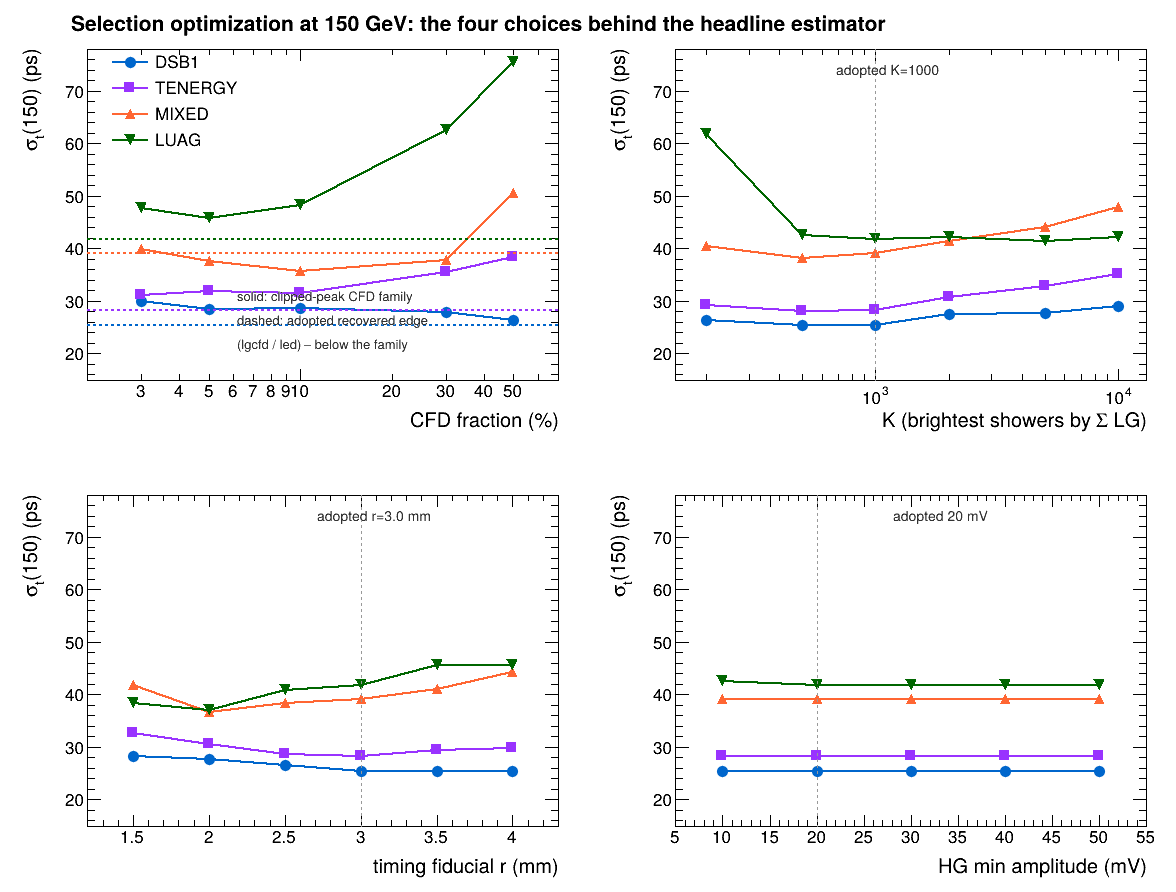
\includegraphics[width=\linewidth]{optimization.png}
\caption{Selection optimization at $150$~GeV for all four builds: (a) timing source as a
function of CFD fraction on the clipped peak (solid) with the adopted recovered-edge
source overlaid (dashed); (b) resolution versus the brightest-$N$ selection $K$;
(c) versus timing fiducial radius; (d) versus the per-channel HG threshold. Dashed grey
lines mark the adopted working points.}
\label{fig:opt}
\end{figure}

\begin{figure}[t]
\centering

\includegraphics[width=\linewidth]{systematics.png}
\caption{Systematic stability of the brightest-$1000$ $\sigma_t(150)$ for each build: the
nominal value (star) with its total-systematic band, and each selection variation as a
point. The fitted floor $b$ with its statistical and systematic errors is annotated per
build. All variations lie within the band except the deliberate $K=2000$ loosening of
the brightness selection.}
\label{fig:syststab}
\end{figure}

%======================================================================
\section*{Acknowledgements}
We thank the CERN SPS staff for the test-beam operation. %% TODO: funding/agency text.

\begin{thebibliography}{9}
\bibitem{cmsmtd} CMS Collaboration, \textit{A MIP Timing Detector for the CMS Phase-2
Upgrade}, Technical Design Report CERN-LHCC-2019-003 (2019).
\bibitem{radical} C.~Perez-Lara, J.~Wetzel, U.~Akgun, et al. (RADiCAL Collaboration),
\textit{Study of time resolution measurements and prospects for energy resolution of
an ultra-compact sampling calorimeter (RADiCAL) module at EM shower maximum over the
energy range 25~GeV--150~GeV}, Nucl. Instrum. Methods A \textbf{1068} (2024) 169737.
\bibitem{drs4} S.~Ritt, R.~Dinapoli, U.~Hartmann, \textit{Application of the DRS chip
for fast waveform digitizing}, Nucl. Instrum. Methods A \textbf{623} (2010) 486--488.
\bibitem{luag} C.~Hu, et al., \textit{LuAG ceramic scintillators for future HEP
experiments}, Nucl. Instrum. Methods A \textbf{954} (2020) 161723.
\end{thebibliography}

\end{document}
